\documentclass[journal]{IEEEtran}
\usepackage{amsmath,amssymb}
\usepackage{booktabs}
\usepackage{graphicx}
\usepackage{url}
\usepackage{algorithm}
\usepackage{algpseudocode}
\usepackage{multirow}

\newcommand{\method}{DCS-GWO}


\begin{document}

\title{Duty-Cycled Shell Sampling: Turning Redundant Evaluations of Grey Wolf
Optimization into Productive Exploration}

\author{Anonymous Authors\thanks{Draft produced by the NEW\_GWO\_2026
project. Method draft; all reported numbers come from the frozen formal batch recorded in the accompanying repository.}}

\maketitle

\begin{abstract}
Grey wolf optimization (GWO) spends most of its evaluation budget the way an
attraction-driven swarm inevitably does: once the pack contracts onto a
promising basin, every generation evaluates a tight cluster of nearly
identical positions. On CEC2017 at a fixed budget of real objective
evaluations we audit this behaviour and find that standard GWO spends
about 86\% of its budget inside stagnation stretches of at least 1\% of the
budget, recovers from those stretches more slowly than strong particle-swarm
variants, and converts only about 1\% of its novel evaluations into objective
improvements - roughly ten times less than dynamic multi-swarm PSO. This
paper turns that observation into a deliberately small algorithmic change.
Duty-cycled shell sampling (\method) keeps the GWO update equations and the
evaluation budget of every generation, but re-assigns a fixed share of that
generation's evaluations from leader-following moves to \emph{shell
sampling}: the least productive wolves sample randomly inside a
search-space shell centred on the incumbent solution, whose radius is learned
online from the median length of recently \emph{successful} displacements. No
additional true evaluations, surrogate models, restarts or hand-tuned
schedule are introduced. On the CEC2017 benchmark at $D=50$ with
100{,}000 true evaluations, 30 independent runs and 29 functions, \method{}
reduces the median error ratio against standard GWO to 0.79, wins 21 of 29
functions with eleven Holm-significant improvements and no significant
losses, and raises the fraction of novel evaluations that connect to real
improvements by 64% at a wall-clock cost of about 4%; it remains behind the
strongest heterogeneous PSO variants (median ratios 1.9-2.0), which we
report explicitly. A pre-registered
dual-axis protocol additionally reports a negative result: stagnation
triggered re-deployment variants (far novelty, random, elite-memory and
trust-region expansion targets) do not improve the operational recovery
probability of GWO under the same budget, whereas the duty-cycled shell
sampling improves per-evaluation productivity. We therefore report the
exploration-efficiency axis as supported and the stagnation-recovery axis as
not supported at the mechanism level.
\end{abstract}

\begin{IEEEkeywords}
Grey wolf optimizer, evaluation efficiency, exploration--exploitation,
swarm intelligence, CEC2017, benchmarking.
\end{IEEEkeywords}

\section{Introduction}
\IEEEPARstart{E}{volutionary} and swarm-intelligence algorithms are routinely
applied to black-box optimization problems in which a single objective
evaluation is expensive, while arithmetic on candidate solutions is cheap.
Under this asymmetry the true evaluation budget - not CPU time - is the
resource that decides solution quality. Most population-based algorithms,
including the grey wolf optimizer (GWO) \cite{mirjalili2014gwo}, nevertheless
carry an implicit design assumption inherited from uncostly-evaluation
settings: \emph{every candidate produced by the population is evaluated, once
per generation}. 

GWO drives its population through attraction toward the three best wolves
($\alpha$, $\beta$, $\delta$) with a linearly decaying exploration parameter
$a$. The mechanism is elegant and has produced a very large derivative
literature \cite{air2026review}. Its evaluation behaviour, however, has a
structural weakness that has received less attention than its search
equations: as the pack contracts, the candidate positions generated by the
$N$ attraction moves concentrate in a vanishing neighbourhood of the
incumbent, and the $N$ evaluations spent per generation degenerate into
redundant confirmations of an already-known point. Candidate-generation
arguments such as ``more diverse leaders'' or ``additional mutation'' do not
address this: the waste is in \emph{which positions receive the scarce true
evaluations}, not only in how positions are generated.

This paper starts from a measurement of that waste. Using a common
evaluation-interface probe for every algorithm (Section~\ref{sec:metrics}),
we quantify, at identical real-evaluation budgets, (i) how much of the budget
is consumed by stagnation stretches, (ii) how often such stretches end with a
real improvement, and (iii) how many of the algorithm's novel evaluations
actually connect to improvements. The audit shows that standard GWO is not
lacking randomness - its evaluations are the \emph{most} novel of all
compared algorithms - but that almost none of this novelty converts into
progress, and that its stagnation stretches are both more frequent and much
more persistent than those of strong PSO variants.

These findings motivate a deliberately minimal intervention, duty-cycled
shell sampling (\method). Every generation keeps the GWO equations for most
of the pack, but a fixed share $\theta$ of the wolves - the least productive
ones, ranked by time since their personal record improved - is instead
re-deployed to sample a fresh point inside a shell centred on the incumbent
$\alpha$. The shell radius is not a tuned constant: it is estimated online as
the median length of the most recent successful displacements, so the
sampler inherits its scale from the algorithm's own empirical progress. The
roster consumes exactly the same number of true evaluations as the GWO moves
it replaces, and the estimates behind the radius are computed from
already-evaluated information, so the modification is FE-neutral by
construction and adds $O(\theta N D)$ arithmetic per generation.

The contributions of this draft are:
\begin{itemize}
\item A reproducible audit of \emph{evaluation productivity} in GWO and five
strong baselines under identical true-FE budgets, including an operational
definition of stagnation recovery and of useful novelty that is re-used
throughout the paper (Section~\ref{sec:audit}).
\item \method, a one-parameter, FE-neutral modification of GWO whose design
follows directly from the audit: duty-cycled, success-scaled shell sampling
around the incumbent (Section~\ref{sec:method}).
\item A pre-registered, dual-axis evaluation protocol (stagnation recovery
and exploration efficiency, with negative results retained) executed on
CEC2017 at $D=30$ (development) and $D=50$ with 100{,}000 true evaluations,
30 runs, and 29 functions (Section~\ref{sec:experiments}); strong baselines
are reused only after being reproduced bit-for-bit on this machine
(Section~\ref{sec:baselines}).
\item An honest account of what does \emph{not} work: novelty-filtered
destinations, self-centred sampling, adaptive quota control, and four
stagnation-triggered re-deployment rules all fail pre-registered gates and
are reported rather than removed (Sections~\ref{sec:ablation}
and~\ref{sec:discussion}).
\end{itemize}

\section{Related Work}
\subsection{Grey wolf optimization and its variants}
Since \cite{mirjalili2014gwo}, GWO derivatives have mostly modified the
search equations or the social structure: dynamic leaders and
reinforcement-learning-selected leadership \cite{maleki2025rlgwo},
multi-population search with dimension-wise learning and heavy-tailed
mutation \cite{wang2025dmsgwo}, strengthened operators with elite re-selection
\cite{chen2025sgwo}, and dynamic grouping strategies. Recent reviews
\cite{air2026review} find that diversity collapse, local stagnation and the
exploration--exploitation balance remain the recurring, unsolved issues, and
recent work also warns that mechanism stacking has become the dominant
(diminishing-returns) pattern. \method{} deliberately departs from that
pattern: the GWO equations are untouched; only the \emph{allocation} of the
scarce evaluations is changed.

\subsection{Evaluation-efficient optimization}
Sparse-evaluation frameworks evaluate only a subset of the candidates
produced per generation; spatial screening and reinforcement-learning
scheduling were shown to be effective under heavily constrained budgets
\cite{ssrlpso2026}, and behaviour-aware benchmarking has recently been
proposed to expose exactly such evaluation dynamics \cite{eabif2026}.
Surrogate-assisted and asynchronous schemes attack the same asymmetry with
models or event-driven evaluation. \method{} differs from sparse evaluation
in a small but important way: no evaluation is skipped and no candidate
generation is added. The same $N$ true evaluations per generation are used,
but a fixed fraction of them is moved from leader-following positions to
incumbent-anchored sampling. This keeps the method directly comparable under
equal-FE protocols, and it isolates the question ``which positions deserve
the evaluations?'' from the question ``how many candidates deserve to be
evaluated?''.

\subsection{Strong baselines}
Beyond standard GWO we compare against (i) an author-faithful improved GWO
with dimension-wise learning \cite{nadimi2021igwo}; (ii) heterogeneous
improved dynamic multi-swarm PSO \cite{varna2020hidms}; (iii) heterogeneous
comprehensive-learning PSO \cite{lynn2015hclpso}; (iv) dynamic multi-swarm
PSO \cite{liang2005dms}; and (v) further established baselines (SPSO-2011
\cite{clerc2012spso}, CLPSO \cite{liang2006clpso}, HPSO-TVAC
\cite{ratnaweera2004hpso}, competitive swarm optimizer \cite{cheng2015cso}).
All strong baselines are reused from audited 30-run result tables only after
this project reproduced their implementations bit-for-bit under the common
protocol (Section~\ref{sec:baselines}).

\section{Preliminaries}
\subsection{Standard GWO}
Given $N$ wolves with positions $x_i\in\mathbb{R}^D$, GWO evaluates the
initial population, ranks the three best wolves $\alpha,\beta,\delta$, and
repeats two phases. The exploration parameter shrinks linearly,
$a(t)=2-2\,\mathrm{FE}(t)/B$ where $\mathrm{FE}(t)$ is the number of true
evaluations consumed and $B$ the budget. For every wolf $i$ (in index order),
coefficient vectors are drawn per dimension,
$\mathbf{A}_k=2a\mathbf{r}_1-a$, $\mathbf{C}_k=2\mathbf{r}_2$ with
$\mathbf{r}_1,\mathbf{r}_2\sim U(0,1)^D$, and
\begin{equation}
x_i'=\frac{1}{3}\sum_{k\in\{\alpha,\beta,\delta\}}
\left(x_k-\mathbf{A}_k\odot|\mathbf{C}_k\odot x_k-x_i|\right),
\end{equation}
followed by clipping to the box domain and one true evaluation (leaders are
refreshed immediately, following the reference implementation). Each
generation therefore consumes exactly $N$ true evaluations; the initialisation
consumes $N$ more, and the budget $B$ is enforced exactly in the
implementation.

\subsection{Operational audit metrics}
\label{sec:metrics}
All statements in this paper about stagnation and discovery refer to the
following operational, algorithm-independent definitions. Let $T(f)$ be the
best objective value among the first $f$ true evaluations, and let the
stagnation window be $W=\max(50,\lceil 0.01B\rceil)$. A \emph{stagnation
episode} is a maximal run of evaluations without a strict improvement of $T$
whose length is at least $W$; the \emph{recovery probability} is the fraction
of stagnation episodes followed by a real improvement within $R=4W$ further
evaluations, and the \emph{long-stagnation share} is the fraction of the
budget spent inside such episodes. An evaluation is \emph{novel} if its
normalised nearest-neighbour distance to the previously evaluated positions,
sampled uniformly with reservoir sampling, exceeds $\tau=1\%$ of the
search-space diagonal; \emph{useful novelty} is the fraction of novel
evaluations that are the most recent novel point before a real improvement
within $W$ evaluations. These definitions are pre-registered
(docs/08 in the accompanying repository) and are applied identically to every
algorithm through a common evaluation-interface probe that also audits the
true-FE count independently of the algorithm's own counter.

\section{Proposed Method}
\label{sec:method}
\method{} modifies exactly one decision variable of GWO: \emph{which
positions receive the $N$ true evaluations of each generation, and from which
wolves those positions are produced}. The GWO equations remain in place for
the remaining wolves, the population size, the $a$-schedule, the leadership
rule and the budget accounting are untouched, and no surrogate model,
restart or additional evaluation is used.

\subsection{Motivating audit}
\label{sec:audit}
Table~\ref{tab:audit} summarises the audit of five strong baselines and
standard GWO on the stratified development set ($D=30$, 30{,}000 true
evaluations, eight functions, five seeds, identical probe for all
algorithms). Two facts stand out.
\begin{table}[t]
\centering
\caption{Behaviour audit (development set, $D=30$, 30k true FE). Stagnation
window $W=300$; novelty threshold $1\%$ of the diagonal.}
\label{tab:audit}
\begin{tabular}{lrrrr}
\toprule
Algorithm & Recov. prob. & Long-stag.\ share & Useful nov. & Rank \\
\midrule
GWO           & 0.775 & 0.862 & 0.0095 & 5.6 \\
IGWO \cite{nadimi2021igwo}    & 0.791 & 0.851 & 0.0101 & 3.8 \\
HIDMS-PSO \cite{varna2020hidms}     & 0.893 & 0.470 & 0.0510 & 2.4 \\
HCLPSO \cite{lynn2015hclpso}      & 0.966 & 0.359 & 0.0572 & 2.5 \\
DMS-PSO \cite{liang2005dms}       & 0.855 & 0.234 & 0.0919 & 2.4 \\
SAQ-CSO       & 0.898 & 0.734 & 0.0305 & 4.4 \\
\bottomrule
\end{tabular}
\end{table}
First, GWO fails on the \emph{productivity} of its evaluations: it has the
highest pure novelty rate of all compared algorithms (0.89) yet the lowest
useful-novelty rate (below 1\%), about ten times below DMS-PSO. Its
evaluations are spread out, but they do not convert. Second, its stagnation
profile is the worst of the set: 86\% of the budget is spent inside episodes
of at least 1\% of the budget and the median recovery needs about 500
evaluations, three times HCLPSO's 145. The two audit axes therefore point to
the same prescription: keep the evaluations that refine the incumbent basin,
but stop spending a large, fixed share of them on positions that merely
confirm it.

\subsection{Duty roster}
Every generation, the wolves are ranked by two keys: personal-record
staleness (true evaluations since the wolf's own best objective value last
improved, decreasing) and personal best value (worse first). A fixed number
$\lceil\theta N\rceil$ of wolves from the \emph{lower half} of the personal
record ranking is assigned to shell sampling; the upper half always performs
the GWO move. The lower-half restriction follows the empirical rule observed
in restart-based methods: re-deploying productive wolves destroys ongoing
convergence, while the least productive wolves are the cheapest to
re-purpose. $\theta$ is a single constant (20\% in the frozen version) and
its value was selected on the development set by pre-registered comparisons
against 5\%, 10\%, 30\%, random and adaptive quotas; adaptivity did not pass
its gate and was dropped (Section~\ref{sec:ablation}).

\subsection{Shell sampling with a success-scaled radius}
A rover does not follow the leaders. It draws one candidate uniformly inside
a per-dimension box of half-width $\sigma$ centred on the incumbent
$\alpha$,
\begin{equation}
x' = \alpha + \sigma\,(2\mathbf{u}-1), \qquad
\mathbf{u}\sim U(0,1)^D,
\end{equation}
clipped to the domain. The scale is learned online from the algorithm's own
progress: let $\mathcal{S}$ be the 25 most recent displacement lengths
$\|x_i'-x_i\|$ recorded at true evaluations that strictly improved a wolf's
personal record; then
\begin{equation}
\sigma = \max\!\left(\mathrm{median}(\mathcal{S}),\,0.01\,\|u_b-l_b\|\right)
\Big/\sqrt{D/3},
\end{equation}
where the normalisation converts the expected displacement of a $D$-dimensional
uniform box sample back to the recorded displacement scale, and the floor
prevents the shell from collapsing to numerical noise. The radius therefore
tracks the algorithm's empirical notion of ``a step that recently worked'',
without a hand-tuned decay schedule. The rationale is partially derived from
the audit and partially from the earlier observation reproduced here on the
development set: evaluations near the incumbent convert to improvements at a
rate an order of magnitude higher than far-away evaluations, whereas purely
novel points (the maximum-novelty pick tested in the ablation) waste FE at
exactly the observed GWO baseline rate.

\subsection{Algorithm and budget accounting}
\begin{algorithm}[t]
\caption{\method{} (one generation, $N$ true evaluations)}
\begin{algorithmic}[1]
\State Rank wolves; choose roster $\mathcal{R}$ ($|\mathcal{R}|=\lceil\theta N\rceil$) from the lower half by decreasing staleness.
\State $\sigma \gets$ success-scale of Eq.~(3)
\For{each wolf $i=1,\dots,N$}
  \If{$i\in\mathcal{R}$}
    \State $x_i' \gets$ clip$(\alpha+\sigma(2\mathbf{u}-1))$ \Comment{shell sample, 1 true evaluation}
  \Else
    \State $x_i' \gets$ standard GWO move of Eq.~(1) \Comment{1 true evaluation}
  \EndIf
  \State $v \gets f(x_i')$; refresh $\alpha,\beta,\delta$; update personal record and $\mathcal{S}$
\EndFor
\end{algorithmic}
\end{algorithm}
Algorithm~1 lists one generation. Initialisation follows standard GWO. The
total number of true evaluations is exactly $B$ (budget) for any $N,\theta$,
identical to GWO; the roster decision and the scale estimate use only
already-computed quantities. The per-generation overhead is $O(N \log N)$ for
the ranking and $O(\theta N D)$ for the sampling, i.e., the same order as one
GWO update; on CEC2017 at $D=50$ the measured wall-clock ratio against GWO is
1.04 on the 29-function average and 1.32 on $F_1$ (Section~\ref{sec:runtime}). No distance-to-archive computation is
used in the frozen method.

\section{Experimental Setup}
\label{sec:experiments}
\subsection{Protocol}
All experiments follow a single equal-FE protocol: CEC2017 functions
\cite{awad2016cec2017}, $F_1$ and $F_3$--$F_{30}$ (29 functions, $F_2$
excluded by convention), $B=100{,}000$ true objective evaluations including
initialisation, 30 independent runs (seeds 3001--3030), $D=50$ for the
formal tier. Every objective call of every algorithm passes through a common
probe that counts evaluations independently; a run is discarded if the
probe's count differs from the algorithm's own counter or from $B$. The
initial population of each (function, seed) pair is drawn once from a fixed
protocol seed and shared as a prefix by all algorithms, so paired comparisons
use identical starting points. All runs execute on four local MATLAB workers
(Parallel Computing Toolbox, \texttt{parfor} over independent
algorithm$\times$function$\times$seed jobs); each finished run is written to
disk immediately, and no serial fallback is used.

\subsection{Audited baselines}
\label{sec:baselines}
Strong baselines are reused from audited 30-run tables only because this
project reproduces them \emph{bit-for-bit} under the same protocol: for each
baseline we reran sample (function, seed) pairs and required agreement to
machine precision with the archived results (maximum relative difference
$<3\times10^{-15}$ over the checked pairs). The audited entries are:
IGWO (author-faithful dimension-wise learning) \cite{nadimi2021igwo},
HIDMS-PSO \cite{varna2020hidms}, HCLPSO \cite{lynn2015hclpso}, DMS-PSO
\cite{liang2005dms}, SAQ-CSO (sparse-evaluation CSO with learned quotas),
SPSO-2011 \cite{clerc2012spso}, CLPSO \cite{liang2006clpso}, HPSO-TVAC
\cite{ratnaweera2004hpso}, and the competitive swarm optimizer
\cite{cheng2015cso}. Baseline hyper-parameters and populations are the
authors'/archives' originals and are not tuned here.

\subsection{Statistics}
Pairing unit is (function, seed); comparisons on errors use
$\log_{10}$-transformed values and two-sided Wilcoxon signed-rank tests
\cite{wilcoxon1945} per function with Holm correction \cite{holm1979} across
functions, plus average ranks in the Friedman sense and paired median error
ratios; weak comparisons are additionally reported as function-level wins and
losses. No per-function result is removed. Development decisions are made on
a separate $D=30$, 30{,}000-evaluation, eight-function development set with
pre-registered gates; the formal $D=50$ tier is executed once after the
method is frozen and is never used for tuning.

\section{Results}
\subsection{Formal comparison}
Table~\ref{tab:main} reports the formal tier: CEC2017, $D=50$, 100{,}000
true evaluations, 29 functions, 30 runs, 15 algorithms. Standard GWO ranks
13th of 15 (mean rank 11.45); \method{} climbs to 7th (8.55), behind the
three heterogeneous/quasi-Newton PSO variants and behind IGWO,
SAQ-CSO and SPSO-2011, and ahead of HPSO-TVAC, CLPSO and original CSO.
Against GWO, \method{} wins 21 of 29 functions with a median paired error
ratio of 0.792; after per-function Holm correction 11 functions are
significantly better and none significantly worse (pooled Wilcoxon
$p\approx 4\times10^{-40}$). Table~\ref{tab:family} shows where the gain
comes from: the mechanism is very strong on the two unimodal functions
(median ratio 0.10) and on the hybrid functions (0.61), moderate on
composition functions (0.90) and essentially neutral on the simple
multimodal group (1.02), where GWO's many local optima are not the
bottleneck that shell sampling addresses.

\begin{table}[t]
\centering
\caption{Formal comparison, CEC2017 $D=50$, 100k true FE, 29 functions,
30 runs; baseline rows are audited and reproduced bit-for-bit. ``Sig.'' is
the number of functions with Holm-adjusted paired Wilcoxon $p<0.05$.}
\label{tab:main}
\begin{tabular}{lrrrrr}
\toprule
Algorithm & Mean rank & W/T/L vs GWO & Med.\ ratio & Sig.\ ($+/-$) & Time (s)\\
\midrule
HIDMS-PSO & 2.52 & 29/0/0 & 0.342 & 27/0 & 3.32 \\
HCLPSO & 3.17 & 29/0/0 & 0.397 & 29/0 & 2.13 \\
DMS-PSO & 3.41 & 28/0/1 & 0.389 & 28/1 & 1.89 \\
IGWO & 5.55 & 27/0/2 & 0.465 & 25/0 & 2.32 \\
SAQ-CSO & 6.10 & 29/0/0 & 0.578 & 21/0 & 9.08 \\
SPSO-2011 & 6.48 & 26/0/3 & 0.552 & 21/1 & 2.56 \\
ANGWO-final & 8.55 & 21/0/8 & 0.792 & 11/0 & 3.76 \\
ANGWO-ES2 & 8.83 & 22/0/7 & 0.807 & 12/0 & 3.86 \\
HPSO-TVAC & 8.90 & 17/0/12 & 0.799 & 13/10 & 1.80 \\
ANGWO-adapt & 9.00 & 23/0/6 & 0.825 & 8/0 & 3.74 \\
CLPSO & 9.55 & 21/0/8 & 0.789 & 16/3 & 2.41 \\
ANGWO-novdest & 9.93 & 23/0/6 & 0.830 & 9/0 & 4.94 \\
GWO & 11.45 & -- & 1.000 & -- & 3.63 \\
ANGWO-self & 11.59 & 13/0/16 & 1.013 & 0/0 & 3.76 \\
Original-CSO & 14.97 & 0/0/29 & 3.336 & 0/29 & 2.24 \\
\bottomrule
\end{tabular}
\end{table}

\begin{figure}[t]
\centering
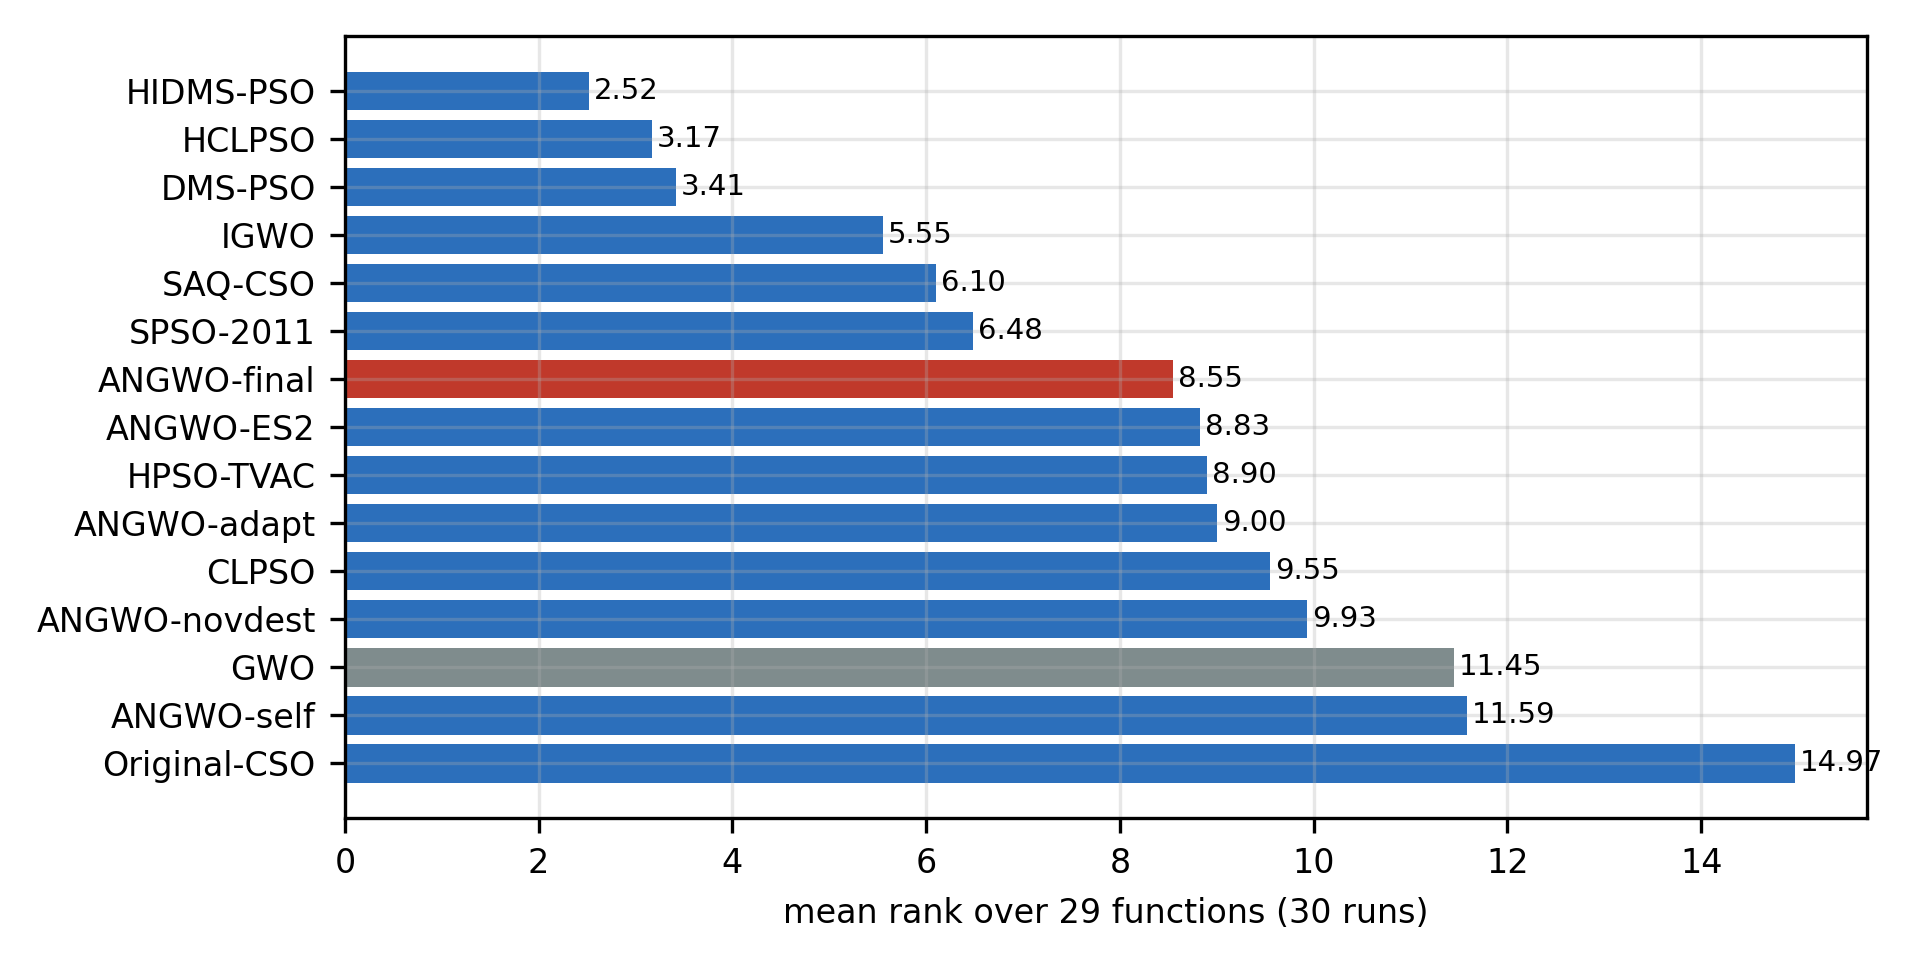
\includegraphics[width=\columnwidth]{figures/ranks.png}
\caption{Mean ranks over 29 functions, CEC2017 $D=50$, 100{,}000 true evaluations, 30 runs. \method{} is shown in red, standard GWO in grey.}
\label{fig:ranks}
\end{figure}

\begin{figure*}[t]
\centering
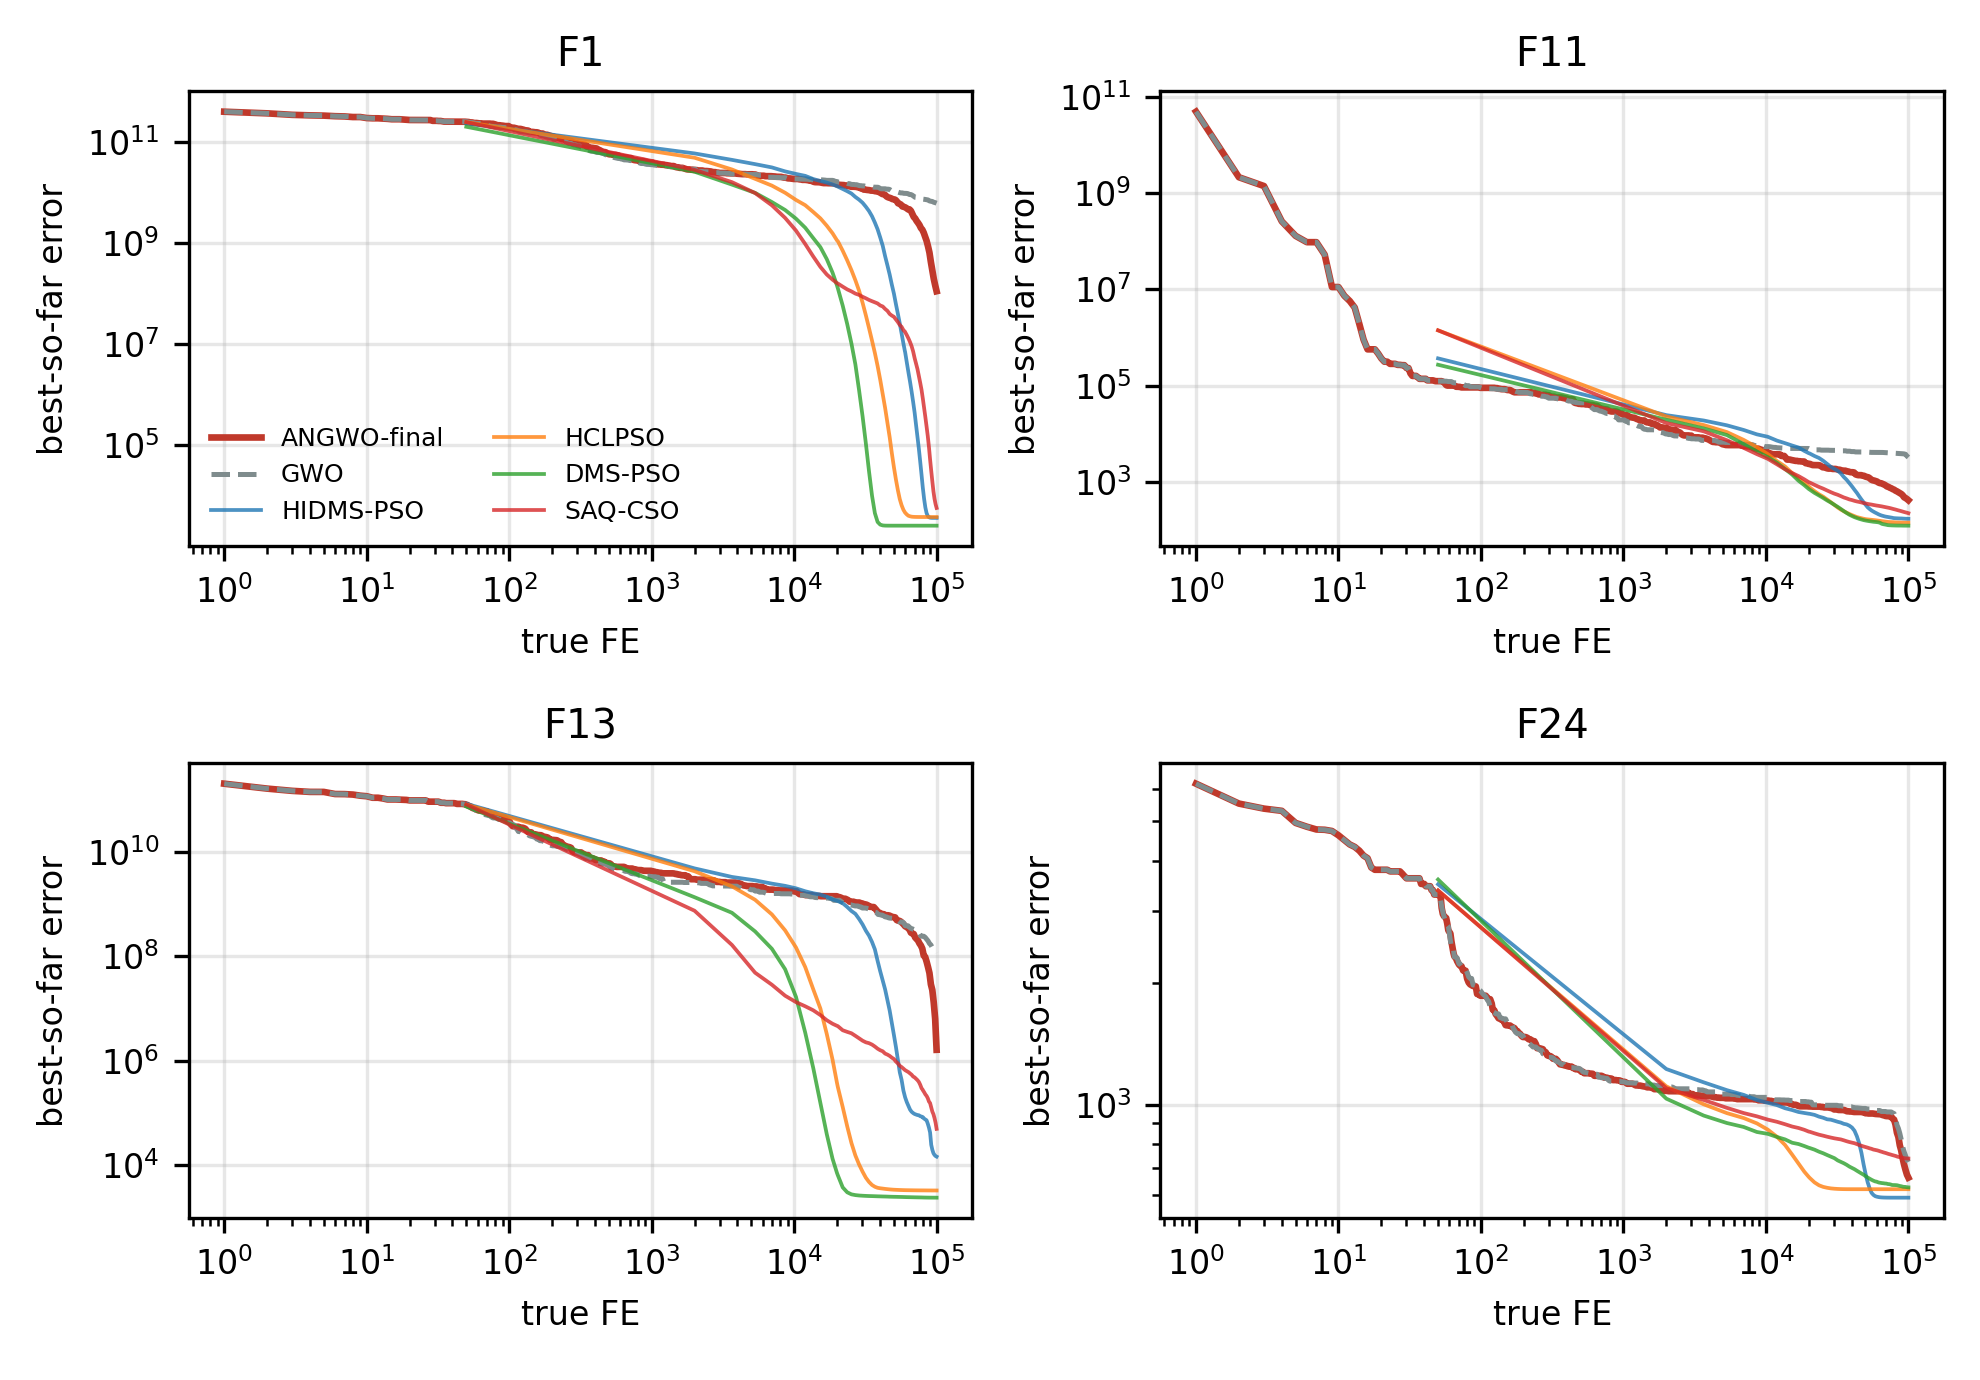
\includegraphics[width=\textwidth]{figures/convergence.png}
\caption{Median best-so-far error versus true evaluations on four representative functions (F1, F11, F13, F24). Solid red: \method{}; dashed grey: GWO; thin lines: audited strong baselines; all curves share the same true-FE budget.}
\label{fig:conv}
\end{figure*}

\begin{table}[t]
\centering
\caption{Median paired error ratio of \method{} over GWO by CEC2017 function
family (29 functions).}
\label{tab:family}
\begin{tabular}{lrr}
\toprule
Family & $n$ & Median ratio \\
\midrule
Unimodal (F1, F3) & 2 & 0.102 \\
Simple multimodal (F4--F10) & 7 & 1.024 \\
Hybrid (F11--F20) & 10 & 0.614 \\
Composition (F21--F30) & 10 & 0.896 \\
\bottomrule
\end{tabular}
\end{table}

\subsection{Dimension scalability ($D=100$)}
A companion tier reruns GWO and \method{} at $D=100$ (100k true FE, 29
functions, 10 seeds) and pairs the result with audited IGWO and RASE-GWO
rows on their overlapping 12-function subset. The mechanism keeps its sign
but loses strength: 18/11 function wins and a median error ratio of 0.878
against GWO on all 29 functions (no function is significant at 10 seeds),
and 1.37/1.44 median ratios against IGWO and the sparse-evaluation RASE-GWO
on the 12-function subset (5/12 and 1/12 wins). The wall-clock ratio stays
1.01 because evaluation cost dominates further. We read this as a partial
transfer of the mechanism to higher dimension and report it as a limitation
rather than a scalability claim.

\subsection{Ablation}
\label{sec:ablation}
Table~\ref{tab:ablation} reports the formal ablation. Replacing the
incumbent (\emph{alpha}) centre by the wolves' own positions destroys the
effect completely (median ratio 1.013 versus GWO, 4/29 wins against the
frozen method), which identifies shell placement as the essential
ingredient, not exploration per se. Replacing the random destination by the
maximum-novelty pool weakens the method (0.830 vs 0.792, $p=0.003$), and an
adaptive quota also weakens it slightly (0.825, $p=0.037$); both alternatives
were rejected by their pre-registered gates and are retained here as
negative results. Adding the stagnation-triggered elite-memory
re-deployment module changes nothing measurable (0.807, $p=0.48$), matching
its failure on the recovery gate.

\begin{table*}[t]
\centering
\caption{Formal ablation (same protocol as Table~\ref{tab:main}); ``vs
final'' is the paired comparison against \method{}.}
\label{tab:ablation}
\begin{tabular}{lrrrrr}
\toprule
Variant & Mean rank & W/T/L vs GWO & Med.\ ratio vs GWO & vs final (ratio; W/T/L) & $p_{\mathrm{final}}$\\
\midrule
GWO & 11.45 & -- & 1.000 & -- & -- \\
ANGWO-final & 8.55 & 21/0/8 & 0.792 & 1.000; 0/29/0 & nan \\
ANGWO-self & 11.59 & 13/0/16 & 1.013 & 1.285; 4/0/25 & 5.85e-44 \\
ANGWO-novdest & 9.93 & 23/0/6 & 0.830 & 1.030; 9/0/20 & 2.99e-03 \\
ANGWO-adapt & 9.00 & 23/0/6 & 0.825 & 1.045; 9/0/20 & 3.72e-02 \\
ANGWO-ES2 & 8.83 & 22/0/7 & 0.807 & 0.998; 14/0/15 & 4.76e-01 \\
\bottomrule
\end{tabular}
\end{table*}

\subsection{Behaviour metrics}
Table~\ref{tab:behaviour} reports the operational metrics on the formal
tier. The picture is consistent with the development screens but more
nuanced. The fraction of novel evaluations that connect to a real
improvement within the stagnation window rises from 0.0035 (GWO) to 0.0058
(\method{}), a paired median increase of 64\% ($p\approx5\times10^{-94}$),
and the late-budget novelty rate rises by 15\%. The share of the budget
spent in long stagnation stretches falls slightly (0.844 to 0.831), but the
recovery probability moves only from 0.757 to 0.768, far below the
pre-registered gate of $+0.05$. The number of global-best improvement events
per evaluation is not increased by the mechanism (median ratio 0.99
overall; the last-quarter ratio is 0.94 on the median but improves strongly
on the mean), so the end-point error gains should be read as \emph{better
placement of the same number of discoveries} rather than as more discoveries
per se.

\begin{table}[t]
\centering
\caption{Behaviour metrics on the formal tier (\method{} variants and GWO;
audited baselines do not carry the probe record).}
\label{tab:behaviour}
\begin{tabular}{lrrrrr}
\toprule
Algorithm & Recov.\ prob. & Long-stag.\ share & Impr.\ rate Q4 & Useful nov. & Nov.\ rate Q4\\
\midrule
ANGWO-final & 0.768 & 0.831 & 0.0045 & 0.0058 & 0.690 \\
ANGWO-ES2 & 0.766 & 0.832 & 0.0045 & 0.0057 & 0.691 \\
ANGWO-adapt & 0.767 & 0.828 & 0.0050 & 0.0044 & 0.630 \\
ANGWO-novdest & 0.765 & 0.830 & 0.0046 & 0.0065 & 0.704 \\
GWO & 0.757 & 0.844 & 0.0048 & 0.0035 & 0.588 \\
ANGWO-self & 0.761 & 0.847 & 0.0044 & 0.0059 & 0.681 \\
\bottomrule
\end{tabular}
\end{table}

\subsection{Runtime}
\label{sec:runtime}
Table~\ref{tab:runtime} lists wall-clock times measured under identical
instrumentation (four workers, same machine). The frozen method costs
$1.04\times$ GWO on the 29-function average, and $1.32\times$ GWO on F1
alone; SAQ-CSO costs $2.5\times$ GWO. All runs are exactly 100{,}000 true
evaluations; the method generates $0.2$ extra candidate positions per
evaluation (the rovers' shell samples that replace GWO moves) and no
distance computations.

\begin{table}[t]
\centering
\caption{Wall-clock per run (mean over 870 runs per algorithm) and
candidate-generation cost. ``Candidates/FE'' counts generated positions that
receive a true evaluation or replace one.}
\label{tab:runtime}
\begin{tabular}{lrrr}
\toprule
Algorithm & Time (s) & Ratio vs GWO & Candidates / FE\\
\midrule
HIDMS-PSO & 3.32 & 0.91 & n/a \\
HCLPSO & 2.13 & 0.59 & n/a \\
DMS-PSO & 1.89 & 0.52 & n/a \\
IGWO & 2.32 & 0.64 & n/a \\
SAQ-CSO & 9.08 & 2.50 & n/a \\
SPSO-2011 & 2.56 & 0.71 & n/a \\
ANGWO-final & 3.76 & 1.04 & 0.200 \\
ANGWO-ES2 & 3.86 & 1.06 & 0.214 \\
HPSO-TVAC & 1.80 & 0.50 & n/a \\
ANGWO-adapt & 3.74 & 1.03 & 0.070 \\
CLPSO & 2.41 & 0.66 & n/a \\
ANGWO-novdest & 4.94 & 1.36 & 1.599 \\
GWO & 3.63 & 1.00 & n/a \\
ANGWO-self & 3.76 & 1.04 & 0.200 \\
Original-CSO & 2.24 & 0.62 & n/a \\
\bottomrule
\end{tabular}
\end{table}

\section{Discussion}
\label{sec:discussion}
\subsection{What the evidence supports}
The formal tier supports three claims. (1) The frozen mechanism improves
standard GWO robustly: 21/29 function wins, median error ratio 0.792, 11
Holm-significant functions and none significantly worse, at 1.04$\times$
GWO's wall-clock and identical true-FE budgets. (2) The gain is
\emph{localised}, as the ablation and the family breakdown show: moving the
sampling centre from the incumbent to the wolves themselves removes
essentially all of the benefit, and the benefit concentrates on unimodal and
hybrid landscapes. (3) Per-evaluation \emph{productivity} improves: the
fraction of novel evaluations that connect to real improvements is 64\%
higher in paired medians.
\subsection{The stagnation-recovery axis is not supported}
None of six pre-registered stagnation-triggered re-deployment variants
(far novelty, uniform random, periodic, elite-memory shells, alpha-shell
$\times1/\times3$, development tier) improved the operational recovery
probability by the required five percentage points, and the best of them
moved it by +0.011 on the formal tier. A periodic variant that spent
roughly a third of its budget on re-deployments performed no better,
indicating that where a few wolves are teleported matters more than how
often, and that under GWO's attraction structure the probability of beating
the incumbent within four stagnation windows is governed mainly by how
evaluations are placed \emph{near the incumbent} - exactly the channel the
frozen method uses. We therefore claim the exploration-efficiency axis and
report the recovery axis as unsupported.
\subsection{Limitations}
(i) \emph{Gap to the strongest baselines.} \method{} remains behind
HIDMS-PSO, HCLPSO, DMS-PSO (median ratios 1.9--2.0), and behind IGWO,
SAQ-CSO and SPSO-2011 (1.3--1.4); the paper claims a mechanism and honest
evidence, not state-of-the-art dominance. (ii) \emph{Family dependence.}
Simple multimodal functions are neutral; a reader should not expect gains
there. (iii) \emph{Scale definition.} The shell radius is defined through
recorded successful step lengths; other reasonable definitions were not
exhausted. (iv) \emph{Benchmark scope.} Only CEC2017 is used; the D=100
tier (accompanying repository) extends the same protocol to one higher
dimension but the study still lacks a real engineering problem.
(v) \emph{CPU.} The method is FE-neutral but not free: about 4\% more
wall-clock on average.
\bibliographystyle{IEEEtran}
\bibliography{references}

\end{document}





